\chapter{Two shortcomings of Korat}
\label{ch:shortcomings-of-korat}
This chapter presents two scenarios where
Korat fails to perform as expected.  The first
example shows how the use of reflection for field accesses may render
Korat unable to generate some valid structures.  The second example
shows how a poorly-written RepOk may adversely affect the performance
of Korat and force it to explore many more states than necessary.
Both examples use a binary tree data structure and implement different
RepOk methods that check the same set of properties but operate
differently.  We compare the performance of Korat by using these RepOk
methods against using the standard binary tree RepOk from Korat
distribution.  Chapter \ref{ch:evaluation} provides experimental
results using additional data structures.

\section{Usage of reflection for field access}
\label{sec:usage-of-reflection-for-field-access}
This example first illustrates how a RepOk method can be written with
and without using reflection for field accesses and then shows how the
output of Korat differs in terms of the sets of valid structures
generated.

\para
Figure \ref{fig:btreeDirectRepOk} shows the Java declaration of a
binary tree and a standard implementation of its RepOk
method\footnote{\url{korat.sourceforge.net}}. Each object of the class
\emph{BinaryTree} represents a binary tree. The value of the
\emph{size} field is the number of nodes in the tree. Objects of the
inner class \emph{Node} represent nodes of the tree.  The RepOk method
performs a traversal of its input object graph and checks that it has
no cycle and the value of the size field is correctly set to the
actual number of nodes reachable from root.  In more detail, first,
\emph{RepOk} checks if the tree is empty. If not, \emph{RepOk} checks
that there are no undirected cycles in the object graph reachable from
the \emph{root} field along the \emph{left} and \emph{right}
fields. It finally checks that the number of nodes reachable from the
root is the same as the value of field \emph{size}.

\begin{figure}
\centering
\begin{lstlisting}[language=Java]
class BinaryTree {
    Node root;    // root node
    int size;    // number of nodes in the tree
    static class Node {
        Node left;    // left child
        Node right;    // right child
    }

    boolean RepOk() {
        // checks that empty tree has size zero.
        if (root == null) return size == 0;
        Set visited = new HashSet();
        visited.add(root);
        LinkedList workList = new LinkedList();
        workList.add(root);
        // loop checks that the object graph is a tree.
        while (!workList.isEmpty()) {
            Node current = (Node) workList.removeFirst();
            if (current.left != null) {
                if (!visited.add(current.left))
                    return false;
                workList.add(current.left);
            }
            if (current.right != null) {
                if (!visited.add(current.right))
                    return false;
                workList.add(current.right);
            }
        }
        // checks that the size is consistent.
        return (visited.size() == size);
    }
}
\end{lstlisting}
\caption{Binary tree example with RepOk using direct field access.}
\label{fig:btreeDirectRepOk}
\end{figure}

\para
Recall, to bound the number of structures generated by Korat, the
programmer provides a finitization that specifies bounds on the number
of objects for different types in the data structures and on the
values in the fields of these objects.  For our binary tree example,
the finitization specifies the maximum number of nodes.  A tree is
considered to be in \emph{scope} $n$, if it has at most $n$ nodes. We
can use integers from 0 to $n$ for the \emph{size} field inside the
\emph{BinaryTree} class.

\para Recall also, given a finitization and a value for scope, Korat
generates all non-isomorphic structures that exist for the scope.  In
our example, two binary trees are isomorphic if a permutation of nodes
exists such that it maps each binary tree to the other.

\begin{figure}
\centering
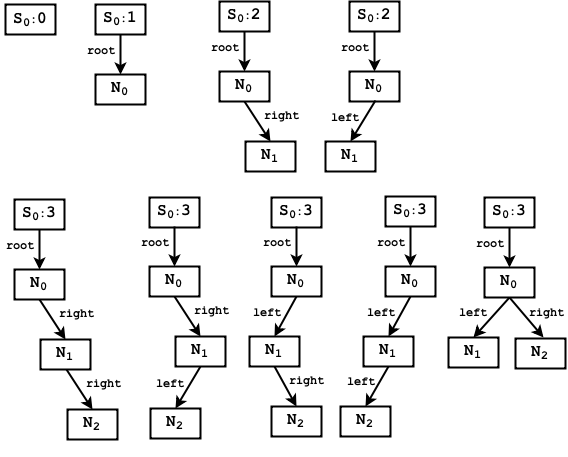
\includegraphics[width=12cm,height=8cm,keepaspectratio]{korat_instances_binary_tree_size_3}
\caption{Binary trees that Korat generates for scope three.}
\label{fig:btreeKoratGenScopeThree}
\end{figure}

\para When using the \emph{RepOk} shown in Figure
\ref{fig:btreeDirectRepOk} with a scope of three, the Korat search
evaluates 90 non-isomorphic candidate structures and outputs 9
structures, which are valid since they satisfy the \emph{RepOk}.
Figure \ref{fig:btreeKoratGenScopeThree} shows the trees that Korat
generates for scope three. Each tree consists of one \emph{BinaryTree}
object $S_0$ and upto three \emph{Node} objects ($N_0$, $N_1$,
$N_2$). For each object, the value and the identity of the \emph{Node}
objects is shown. Edges represent the values of reference fields with
no edge for \emph{null}.

%................................................................

\para To enable efficient search for valid structures, Korat encodes
each structure with a state, and each finitization bounds the state
space. Korat uses backtracking to systematically search this state
space to find all valid structures. Based on a finitization for the
input structures of the predicate, Korat first initializes the state
space of structures. Korat then builds candidate structures and
executes the predicate on them to check their validity. Korat monitors
these executions to dynamically determine which parts of the candidate
the result of the predicate depends on. More specifically, Korat
monitors the fields of the candidates the execution accesses. Korat
monitors field accesses by replacing field accesses with accessor
methods. If the predicate returns \emph{true}, Korat outputs the
candidate as a valid structure for testing. Otherwise, if the
predicate returns false or an exception is thrown in the middle of
execution, Korat skips the candidate. Korat then backtracks on the
values of the accessed fields, to generate the next
candidate. Finally, Korat terminates when it explores the entire
search space.

\begin{figure}
\centering
\begin{lstlisting}[language=Java]
boolean repOK() {
    // checks that empty tree has size zero.
    if (root == null) return size == 0;
    Set visited = new HashSet();
    visited.add(root);
    LinkedList workList = new LinkedList();
    workList.add(root);
    // loop checks that the object graph is a tree.
    while (!workList.isEmpty()) {
        Node current = (Node) workList.removeFirst();
        if ((Node)BinaryTree.class.getDeclaredField(``left'').get(current) != null) {
            if (!visited.add(current.left)) 
                return false;
            workList.add(current.left);
        }
        if (current.right != null) {
            if (!visited.add(current.right))
                return false;
            workList.add(current.right);
        }
    }
    // checks that the size is consistent.
    return (visited.size() == size);
}
\end{lstlisting}
\caption{RepOk using the java reflection API for accessing the left child of a Node inside the loop.}
\label{fig:btTreeReflectionRepOK}
\end{figure}


\begin{figure}
\centering
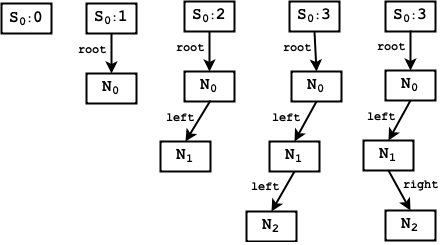
\includegraphics[width=11cm,height=6cm,keepaspectratio]{korat_instances_reflection_binary_tree_size_3}
\caption{ Binary trees that Korat generates for scope three when RepOk uses reflection.}
\label{fig:btreeReflectKoratGenScopeThree}
\end{figure}

\para The main difference between the \emph{RepOk} implementation
shown in figure \ref{fig:btreeDirectRepOk} and the \emph{RepOk}
implementation shown in figure \ref{fig:btTreeReflectionRepOK}) is the
access of just one field. The latter \emph{RepOk} uses the Java
reflection API to access the \emph{left} child of the \emph{Node}
object.  Recall, the use of reflection for field accesses may render
Korat unable to generate some valid structures. Figure
\ref{fig:btreeReflectKoratGenScopeThree} shows the binary tree
structures generated when the RepOk implementation in figure
\ref{fig:btTreeReflectionRepOK} is used to validate the binary tree
candidates that Korat explores. Korat evaluates only 28 non-isomorphic
candidate structures of which 5 structures are output, which are valid
since they satisfy the \emph{RepOk}.


\para Figure \ref{fig:btTreeUserReflectionRepOK} shows another version
of \emph{RepOk} implementation that uses a user written method, which
inturn uses the Java reflection API to access the \emph{left} field of
the \emph{Node}. Though Korat instruments all methods invoked in the
\emph{RepOk}, it will still not be able to monitor accesses that use
reflection even inside another method. Using this version of
\emph{RepOk} implementation to generate binary tree inputs also
produces the same trees shown in figure
\ref{fig:btreeReflectKoratGenScopeThree}.

\begin{figure}
\centering
\begin{lstlisting}[language=Java]
boolean repOK() {
    // checks that empty tree has size zero.
    if (root == null) return size == 0;
    Set visited = new HashSet();
    visited.add(root);
    LinkedList workList = new LinkedList();
    workList.add(root);
    // loop checks that the object graph is a tree.
    while (!workList.isEmpty()) {
        Node current = (Node) workList.removeFirst();
        if ((Node)ReflectionUtils.getFieldValue(current, ``left'') != null) {
            if (!visited.add(current.left))
                return false;
            workList.add(current.left);
        }
        if (current.right != null) {
            if (!visited.add(current.right))
                return false;
            workList.add(current.right);
        }
    }
    // checks that the size is consistent.
    return (visited.size() == size);
}
\end{lstlisting}
\caption{RepOk using the user written reflection API for accessing the left child of a Node inside the loop.}
\label{fig:btTreeUserReflectionRepOK}
\end{figure}


\section{Inefficient predicates}
\label{sec:inefficient-predicates}
Korat efficiently generates all valid non-isomorphic structures even
for large state spaces. The search pruning that Korat performs allows
Korat to explore only a tiny part of the state space. The ratio of the
number of candidate structures evaluated in Korat, to the size of the
state space shows that the key to effective pruning is backtracking
based on fields accessed during predicate execution. Korat performs
efficiently when the user written predicate returns a
\emph{true/false} as soon as it knows the result. Figure
\ref{fig:btreeDirectRepOk} shows a \emph{RepOk} implementation for a
\emph{BinaryTree} returns \emph{false} as soon as it knows that the
candidate has violated one of the three rules for a candidate struture
to be a binary tree.

\para When using the \emph{RepOk} implementation shown in Figure
\ref{fig:btreeDirectRepOk} with a scope of three, Korat evaluates 90
non-isomorphic candidate structures of which 9 structures are
output. The \emph{RepOk} implementation shown in figure
\ref{fig:bTreeInefficient} has the same functionality and also
generates the same valid structures as the \emph{RepOk} implementation
in figure \ref{fig:btreeDirectRepOk} but, it evaluates 893 candidate
structures for scope three which is an order of magnitude more than
the number of candidate structures evaluated by the \emph{RepOk}
implementation in figure \ref{fig:btreeDirectRepOk}. For a larger
scope, we may observe an increase by multiple orders of magnitude. Thus, the
\emph{RepOk} implementation in figure \ref{fig:bTreeInefficient} is
inefficient as it does not return \emph{true/false} right after it
knows the result and therefore makes excessive field accesses.

\begin{figure}
\centering
\begin{lstlisting}[language=Java]
boolean repOK() {
    boolean result = true;
    // checks that empty tree has size zero.
    if (root == null) result = (size == 0);
    Set visited = new HashSet();
    LinkedList workList = new LinkedList();
    if (root != null) {
        visited.add(root);
        workList.add(root);
    }
    // loop checks that the object graph is a tree.
    while (!workList.isEmpty()) {
        Node current = (Node) workList.removeFirst();
        if (current.left != null) {
            if (!visited.add(current.left))
                result = false;
            else workList.add(current.left);
        }
        if (current.right != null) {
            if (!visited.add(current.right)) 
                result = false;
            else workList.add(current.right);
        }
    }
    // checks that the size is consistent.
    if(!result) result = (visited.size() == size);
    return result;
}
\end{lstlisting}
\caption{RepOk that doesn’t return the result as soon as it knows it.}
\label{fig:bTreeInefficient}
\end{figure}
